\documentclass[unknownkeysallowed]{beamer}
\usepackage[french,english]{babel}
\usepackage{sty/beamer_js}
\usepackage{sty/shortcuts_js}

\usepackage{graphicx}
\usepackage{dirtree}
\newcommand{\Benchopt}{\texttt{Benchopt}}

\graphicspath{{/home/temp/Pictures/Logos/}}

\definecolor{tomcolor}{rgb}{0.,.3,.6}
\lstset{basicstyle=\color{tomcolor}\scriptsize\ttfamily}
\addbibresource{../biblio/biblio.bib}
\captionsetup[subfigure]{labelformat=empty}
\begin{document}
\setbeamercovered{invisible}
%%%%%%%%%%%%%%%%%%%%%%%%%%%%%%%%%%%%%%%%%%%%%%%%%%%%%%%%%%%%%%%%%%%%%%%%%%%%%%%
%%%%%%%%%%%%%%%%%%%%%%             Headers               %%%%%%%%%%%%%%%%%%%%%%
%%%%%%%%%%%%%%%%%%%%%%%%%%%%%%%%%%%%%%%%%%%%%%%%%%%%%%%%%%%%%%%%%%%%%%%%%%%%%%%


%%%%%%%%%%%%%%%%%%%%%%%%%%%%%%%%%%%%%%%%%%%%%%%%%%%%%%%%%%%%%%%%%%%%%%%%%%%%%%%
\begin{frame}
\bigskip
\bigskip
\begin{center}{
\LARGE\color{marron}
\textbf{\texttt{Benchopt}:\\
Reproducible, efficient and collaborative optimization benchmarks}
\textbf{ }\\
}

\color{marron}
\end{center}

\vspace{0.5cm}

\begin{center}
\textbf{Reproducible research seminar} \\
\vspace{0.1cm}
Thomas Moreau\\
\end{center}

\centering

\includegraphics[width=0.43\textwidth]{sharedimages/benchopt_logo.pdf}

\end{frame}
%%%%%%%%%%%%%%%%%%%%%%%%%%%%%%%%%%%%%%%%%%%%%%%%%%%%%%%%%%%%%%%%%%%%%%%%%%%%%%%


%%%%%%%%%%%%%%%%%%%%%%%%%%%%%%%%%%%%%%%%%%%%%%%%%%%%%%%%%%%%%%%%%%%%%%%%%%%%%%%
\begin{frame}{A word about me}

    \begin{itemize}\itemsep1em\leftmargin0pt
        \item Researcher at Inria -- MIND
        \item \url{https://tommoral.github.io}
        \item \href{mailto:thomas.moreau@inria.fr}{thomas.moreau@inria.fr}
        \item \textbf{Research topics:} Time-series, Inverse Problems, Bilevel Optimization, Unrolling, Pattern Learning, Point Processes, Physiological signals.
        \item {\large \textbf{OSS maintainer/contributor}\\}
    \end{itemize}
    % \end{minipage}

    \vskip1em\hskip-2em
    \includegraphics[height=4em]{logo_python.png}\hskip.5em
    \includegraphics[height=4em]{logo_sklearn.png}\hskip.5em
    \includegraphics[height=4em]{logo_joblib.png}\hskip.5em
    \includegraphics[height=4em]{logo_loky.png}\hskip.5em
    \includegraphics[height=4em]{logo_benchopt.png}

\end{frame}
%%%%%%%%%%%%%%%%%%%%%%%%%%%%%%%%%%%%%%%%%%%%%%%%%%%%%%%%%%%%%%%%%%%%%%%%%%%%%%%


%%%%%%%%%%%%%%%%%%%%%%%%%%%%%%%%%%%%%%%%%%%%%%%%%%%%%%%%%%%%%%%%%%%%%%%%%%%%%%%
\begin{frame}{Reproducible research}

    Different goals:\\[.5em]
    \begin{itemize}\itemsep.5em
        \item Reproduce the exact same results?
        \item Run with new parameters with robust results?
        \item Run with a new dataset?
        \item Extend the results with a new method?
        \item Provide tools for other to use?
    \end{itemize}
    \vskip2em
    {\centering \large Does not require the same set of tools!\\[2em]}
    % \end{minipage}
    \pause
    {\centering \large Here is my take.\\}


\end{frame}
%%%%%%%%%%%%%%%%%%%%%%%%%%%%%%%%%%%%%%%%%%%%%%%%%%%%%%%%%%%%%%%%%%%%%%%%%%%%%%%


%%%%%%%%%%%%%%%%%%%%%%%%%%%%%%%%%%%%%%%%%%%%%%%%%%%%%%%%%%%%%%%%%%%%%%%%%%%%%%%
\begin{frame}{Reproducing the same results}

    Minimal requirement for a research project:\\[.5em]
    \begin{itemize}\itemsep.5em
        \item Write clean code:
            \begin{itemize}
                \item Consistent style: \emph{Use \texttt{black} or \texttt{flake8}}.
                \item Use readable names.
                \item No notebooks!
            \end{itemize}
        \item Document your code: \emph{docstring and \texttt{README.md}.}
        \item Determinist output: \emph{Set a random seed!}
    \end{itemize}
    \vskip2em
    Optional but advised
    \begin{itemize}\itemsep.5em
        \item Document dependencies.
        \item Proper package organization
        \item Add some tests: \emph{Use \texttt{pytest}.}
    \end{itemize}


\end{frame}
%%%%%%%%%%%%%%%%%%%%%%%%%%%%%%%%%%%%%%%%%%%%%%%%%%%%%%%%%%%%%%%%%%%%%%%%%%%%%%%


%%%%%%%%%%%%%%%%%%%%%%%%%%%%%%%%%%%%%%%%%%%%%%%%%%%%%%%%%%%%%%%%%%%%%%%%%%%%%%%
\begin{frame}{Extending the results?}


    These advice makes it easier to reproduce the same results, but we want to extend them!
    \pause
    \vskip2em

    Pain points of a benchmark:\\[.2em]
    \begin{itemize}
        \item competitors' methods do not work out of the box.
        \item re-code methods and tools to integrate a new method.
        \item hard to extend with new settings.
    \end{itemize}
    \vskip1em
    {\centering \large all of this started from scratch by every submission!\\}
    % \end{minipage}

    \vskip2em


    \Benchopt{} produces \textbf{open}, \textbf{reproducible}, \textbf{extendable} benchmarks

    \end{frame}
    %%%%%%%%%%%%%%%%%%%%%%%%%%%%%%%%%%%%%%%%%%%%%%%%%%%%%%%%%%%%%%%%%%%%%%%%%%%%%%%



%%%%%%%%%%%%%%%%%%%%%%%%%%%%%%%%%%%%%%%%%%%%%%%%%%%%%%%%%%%%%%%%%%%%%%%%%%%%%%%
\begin{frame}{How does \Benchopt{} do it?}

\Benchopt{} is a framework to organize and run benchmarks:
\begin{itemize}
    \item one repository per benchmark
    \item one base open source \texttt{Python} CLI to run them
\end{itemize}

\vskip1em
Examples of existing benchmarks:
\vskip.5em
\begin{minipage}{0.45\linewidth}
    {\small
    \begin{itemize}
        \item Resnet18
        \item Lasso
        \item ICA
        \item Logistic regression
    \end{itemize}
    }
\end{minipage}
\begin{minipage}{0.48\linewidth}
    {\small
    \begin{itemize}
        \item Total Variation
        \item Ordinary Least Squares
        \item Non convex sparse regression
        \item linear SVM
    \end{itemize}
    }
\end{minipage}
\vskip2em

\centering
Start yours with \url{https://github.com/benchopt/template_benchmark}!
\end{frame}
%%%%%%%%%%%%%%%%%%%%%%%%%%%%%%%%%%%%%%%%%%%%%%%%%%%%%%%%%%%%%%%%%%%%%%%%%%%%%%%


%%%%%%%%%%%%%%%%%%%%%%%%%%%%%%%%%%%%%%%%%%%%%%%%%%%%%%%%%%%%%%%%%%%%%%%%%%%%%%%
\begin{frame}{Components of a benchmark}

    \centering
    \vspace*{-5mm}
    \textbf{3 components}: Objective, Dataset, Solver

    \vskip3em
    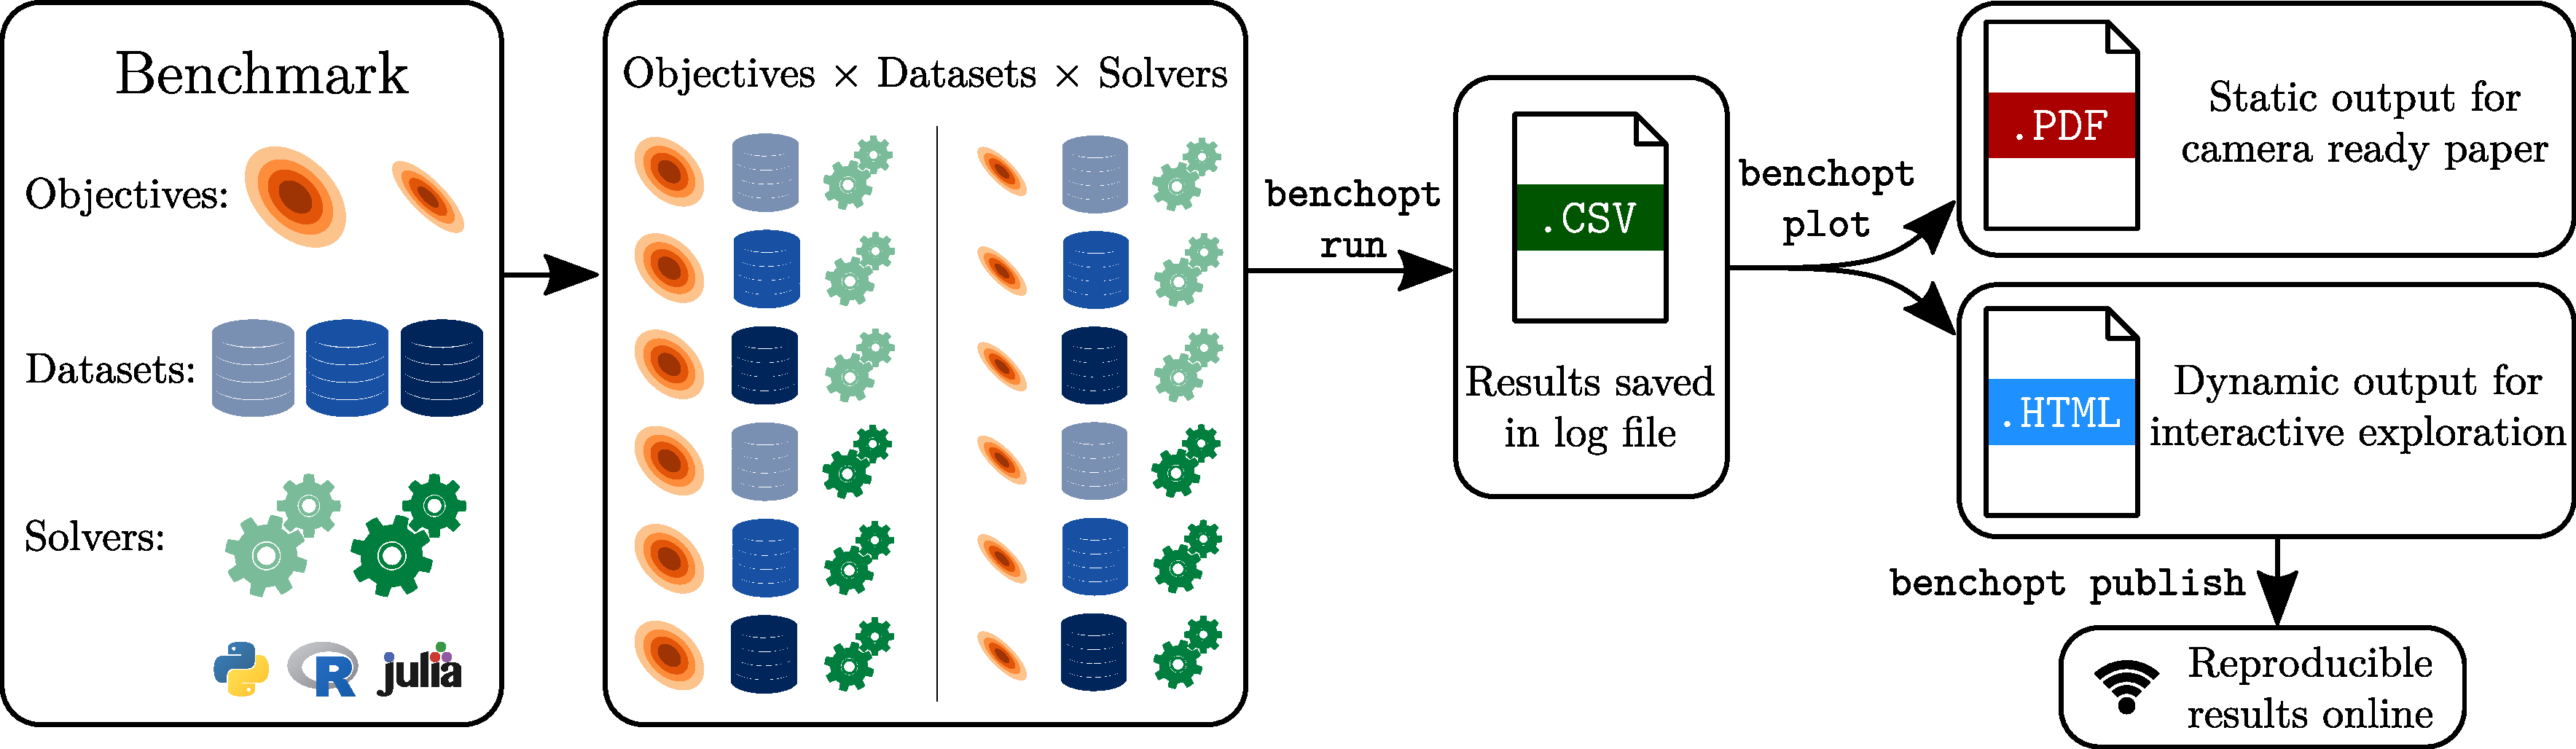
\includegraphics[width=\linewidth]{sharedimages/benchopt_schema.pdf}

\end{frame}
%%%%%%%%%%%%%%%%%%%%%%%%%%%%%%%%%%%%%%%%%%%%%%%%%%%%%%%%%%%%%%%%%%%%%%%%%%%%%%%



%%%%%%%%%%%%%%%%%%%%%%%%%%%%%%%%%%%%%%%%%%%%%%%%%%%%%%%%%%%%%%%%%%%%%%%%%%%%%%%
\begin{frame}{Structure of a benchmark}

    \begin{minipage}{0.45\linewidth}
        \dirtree{%
        .1 benchmark/.
        .2 objective.py.
        .2 datasets/.
        .3 dataset1.py.
        .3 dataset2.py.
        .2 solvers/.
        .3 solver1.py.
        .3 solver2.py.
    }
    \end{minipage}
    \begin{minipage}{0.45\linewidth}

    \textbf{Modular \& extendable}
    \vspace*{5mm}

    New solver? add a file

    New dataset? add a file

    New metric? modify objective
    \end{minipage}

\end{frame}
%%%%%%%%%%%%%%%%%%%%%%%%%%%%%%%%%%%%%%%%%%%%%%%%%%%%%%%%%%%%%%%%%%%%%%%%%%%%%%%

%%%%%%%%%%%%%%%%%%%%%%%%%%%%%%%%%%%%%%%%%%%%%%%%%%%%%%%%%%%%%%%%%%%%%%%%%%%%%%%
\begin{frame}{Interactive results exploration}
    \centering
    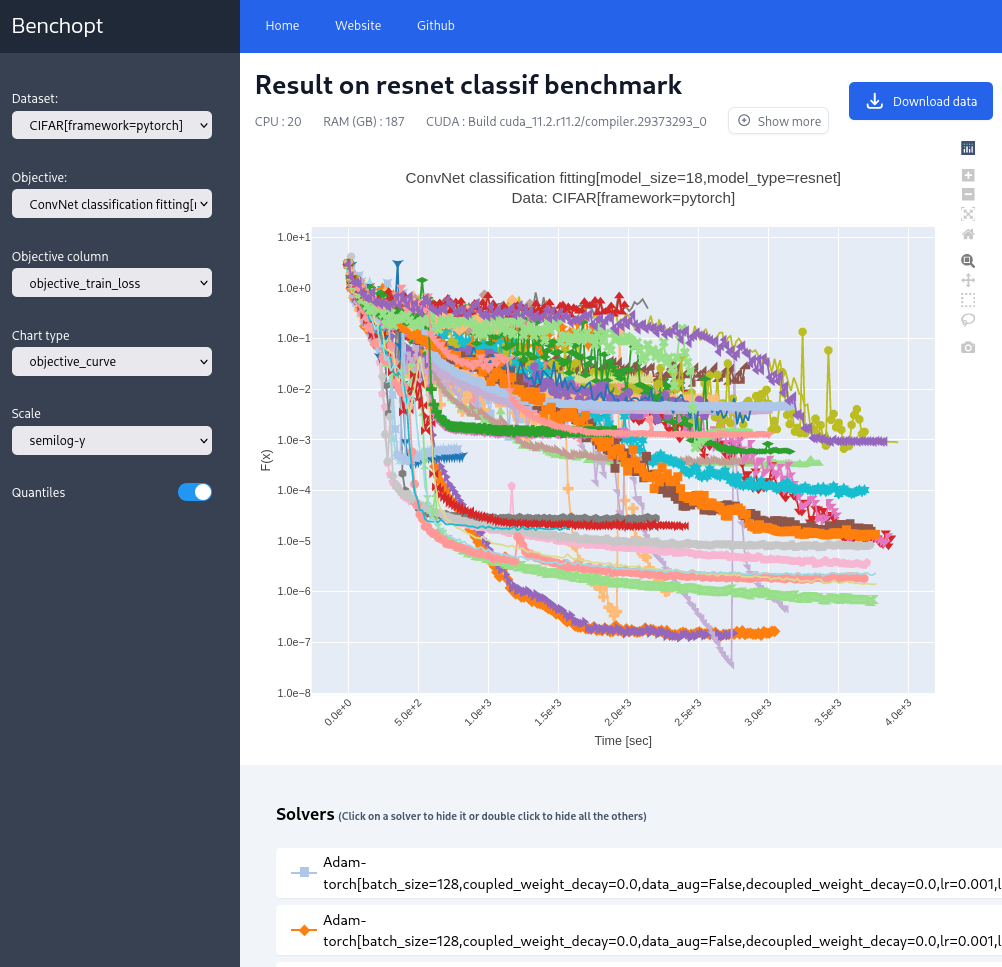
\includegraphics[width=0.8\linewidth]{sharedimages/benchopt_convnet.png}
\end{frame}
%%%%%%%%%%%%%%%%%%%%%%%%%%%%%%%%%%%%%%%%%%%%%%%%%%%%%%%%%%%%%%%%%%%%%%%%%%%%%%%


%%%%%%%%%%%%%%%%%%%%%%%%%%%%%%%%%%%%%%%%%%%%%%%%%%%%%%%%%%%%%%%%%%%%%%%%%%%%%%%
\begin{frame}{\Benchopt{} makes your life easy}

    \begin{itemize}
        \item build on previous benchmarks
        \item use solvers in Python, R, Julia, binaries...
        \item monitor any metric you want altogether (test/train loss, ...)
        \item add parameters to solvers
        \item share and publish HTML results
        \item run all benchmarks in parallel
        \item cache results
        \item and much more!
    \end{itemize}
    \vskip1em
    \centering
    
\includegraphics[width=0.8\linewidth]{sharedimages/tweet_rahimi.png}
\end{frame}
%%%%%%%%%%%%%%%%%%%%%%%%%%%%%%%%%%%%%%%%%%%%%%%%%%%%%%%%%%%%%%%%%%%%%%%%%%%%%%%


%%%%%%%%%%%%%%%%%%%%%%%%%%%%%%%%%%%%%%%%%%%%%%%%%%%%%%%%%%%%%%%%%%%%%%%%%%%%%%%
\begin{frame}{Example: Resnet benchmark}

    { \small
    \begin{itemize}
        \item image classification with resnet18
        \item various optimization strategies
        \item compare \texttt{pytorch} and \texttt{tensorflow}
        \item publish reproducible SOTA for baselines
    \end{itemize}
    }

    \vskip1em
    \centering
    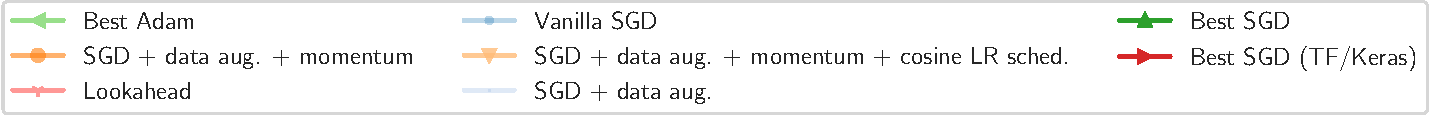
\includegraphics[width=\linewidth]{sharedimages/resnet18_sgd_torch_legend.pdf}
    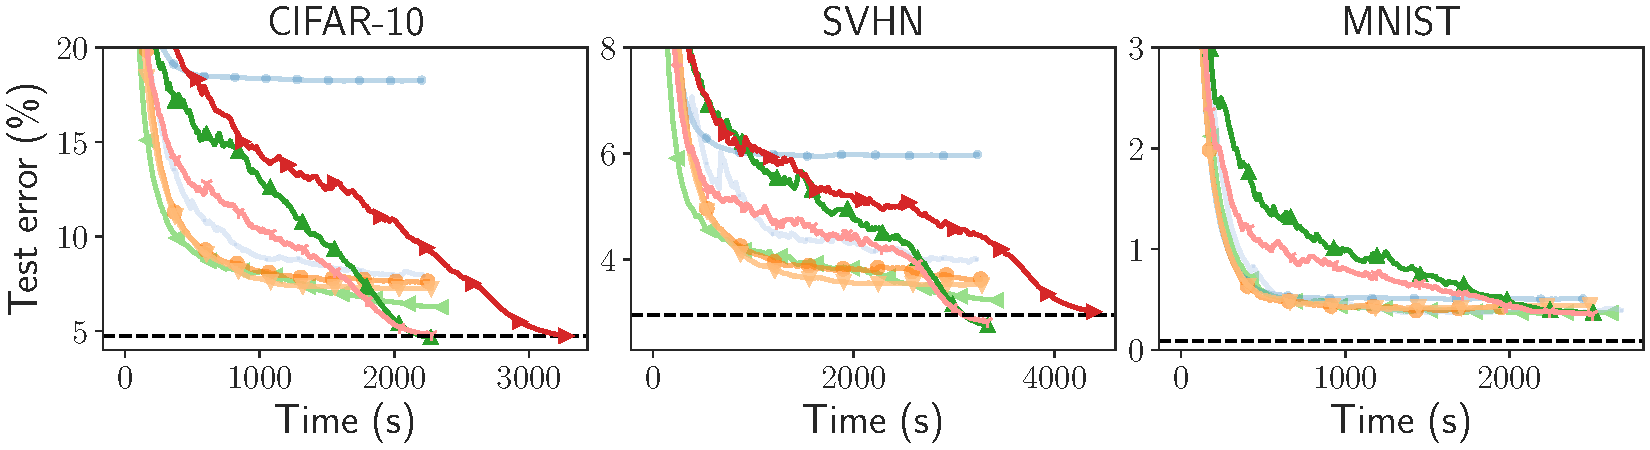
\includegraphics[width=\linewidth]{sharedimages/resnet18_sgd_torch.pdf}

    \url{https://github.com/benchopt/benchmark_resnet_classif/}
\end{frame}
%%%%%%%%%%%%%%%%%%%%%%%%%%%%%%%%%%%%%%%%%%%%%%%%%%%%%%%%%%%%%%%%%%%%%%%%%%%%%%%



%%%%%%%%%%%%%%%%%%%%%%%%%%%%%%%%%%%%%%%%%%%%%%%%%%%%%%%%%%%%%%%%%%%%%%%%%%%%%%%
\begin{frame}{Contributors from...}
    \centering
    
\includegraphics[width=100px]{sharedimages/logo_inria_horiz.pdf} \hspace{1mm}
    
\includegraphics[height=45px]{sharedimages/um_logo.pdf} \hspace{1mm}
    
\includegraphics[height=35px]{sharedimages/logo_berkeley.png} \hspace{1mm}
    \\[7mm]
    
\includegraphics[height=50px]{sharedimages/logo_cnrs.pdf} \hspace{5mm}
    
\includegraphics[height=50px]{sharedimages/logo_lund} \hspace{5mm}
    
\includegraphics[height=50px]{sharedimages/logo_telecom.pdf} \hspace{5mm}
    
\includegraphics[height=50px]{sharedimages/logo_univ_luxembourg.pdf} \\[4mm]
    
\includegraphics[height=40px]{sharedimages/logo_ens.png}
\end{frame}
%%%%%%%%%%%%%%%%%%%%%%%%%%%%%%%%%%%%%%%%%%%%%%%%%%%%%%%%%%%%%%%%%%%%%%%%%%%%%%%



%%%%%%%%%%%%%%%%%%%%%%%%%%%%%%%%%%%%%%%%%%%%%%%%%%%%%%%%%%%%%%%%%%%%%%%%%%%%%%%
\begin{frame}{Benchopt}
    \centering \Huge
    Tutorial: benchmarking iterative solvers.\\[2em]
    \normalsize \url{https://github.com/benchopt/template_benchmark/}
\end{frame}
%%%%%%%%%%%%%%%%%%%%%%%%%%%%%%%%%%%%%%%%%%%%%%%%%%%%%%%%%%%%%%%%%%%%%%%%%%%%%%%


%%%%%%%%%%%%%%%%%%%%%%%%%%%%%%%%%%%%%%%%%%%%%%%%%%%%%%%%%%%%%%%%%%%%%%%%%%%%%%%
\begin{frame}{Going further: creating a package}

    If you really want to make your research \emph{reproductible} by other in different contexts, you need to properly package it.\\[2em]

    \begin{itemize}
        \item Documentation: \emph{Sphinx}.
        \item Test on multiple platforms: \emph{Continuous Integration}.
        \item Release on pypi/conda-forge
        \item Talk about it ! :)
    \end{itemize}

    \vskip2em
    Example of package:
    \url{https://github.com/tomMoral/test_package}


\end{frame}
%%%%%%%%%%%%%%%%%%%%%%%%%%%%%%%%%%%%%%%%%%%%%%%%%%%%%%%%%%%%%%%%%%%%%%%%%%%%%%%


%%%%%%%%%%%%%%%%%%%%%%%%%%%%%%%%%%%%%%%%%%%%%%%%%%%%%%%%%%%%%%%%%%%%%%%%%%%%%%%
\begin{frame}{Conclusion}

    Reproducible research needs more than just releasing code:\\[2em]

    \begin{itemize}
        \item Clean and Documented.
        \item Reusable.
        \item Extendable.
    \end{itemize}

    \vskip2em
    Use proper tools to make it possible!
    \vskip2em
    Research is also collaborative: don't hesitate to report your issues and give feedback :)


\end{frame}
%%%%%%%%%%%%%%%%%%%%%%%%%%%%%%%%%%%%%%%%%%%%%%%%%%%%%%%%%%%%%%%%%%%%%%%%%%%%%%%


%%%%%%%%%%%%%%%%%%%%%%%%%%%%%%%%%%%%%%%%%%%%%%%%%%%%%%%%%%%%%%%%%%%%%%%%%%%%%%%
\begin{frame}{Advertizing}

    Looking for an intern/PhD to join the team!\\[2em]

    \centering
    \includegraphics[width=.4\textwidth]{sharedimages/parietal_karting_deauville.png}
    \hfill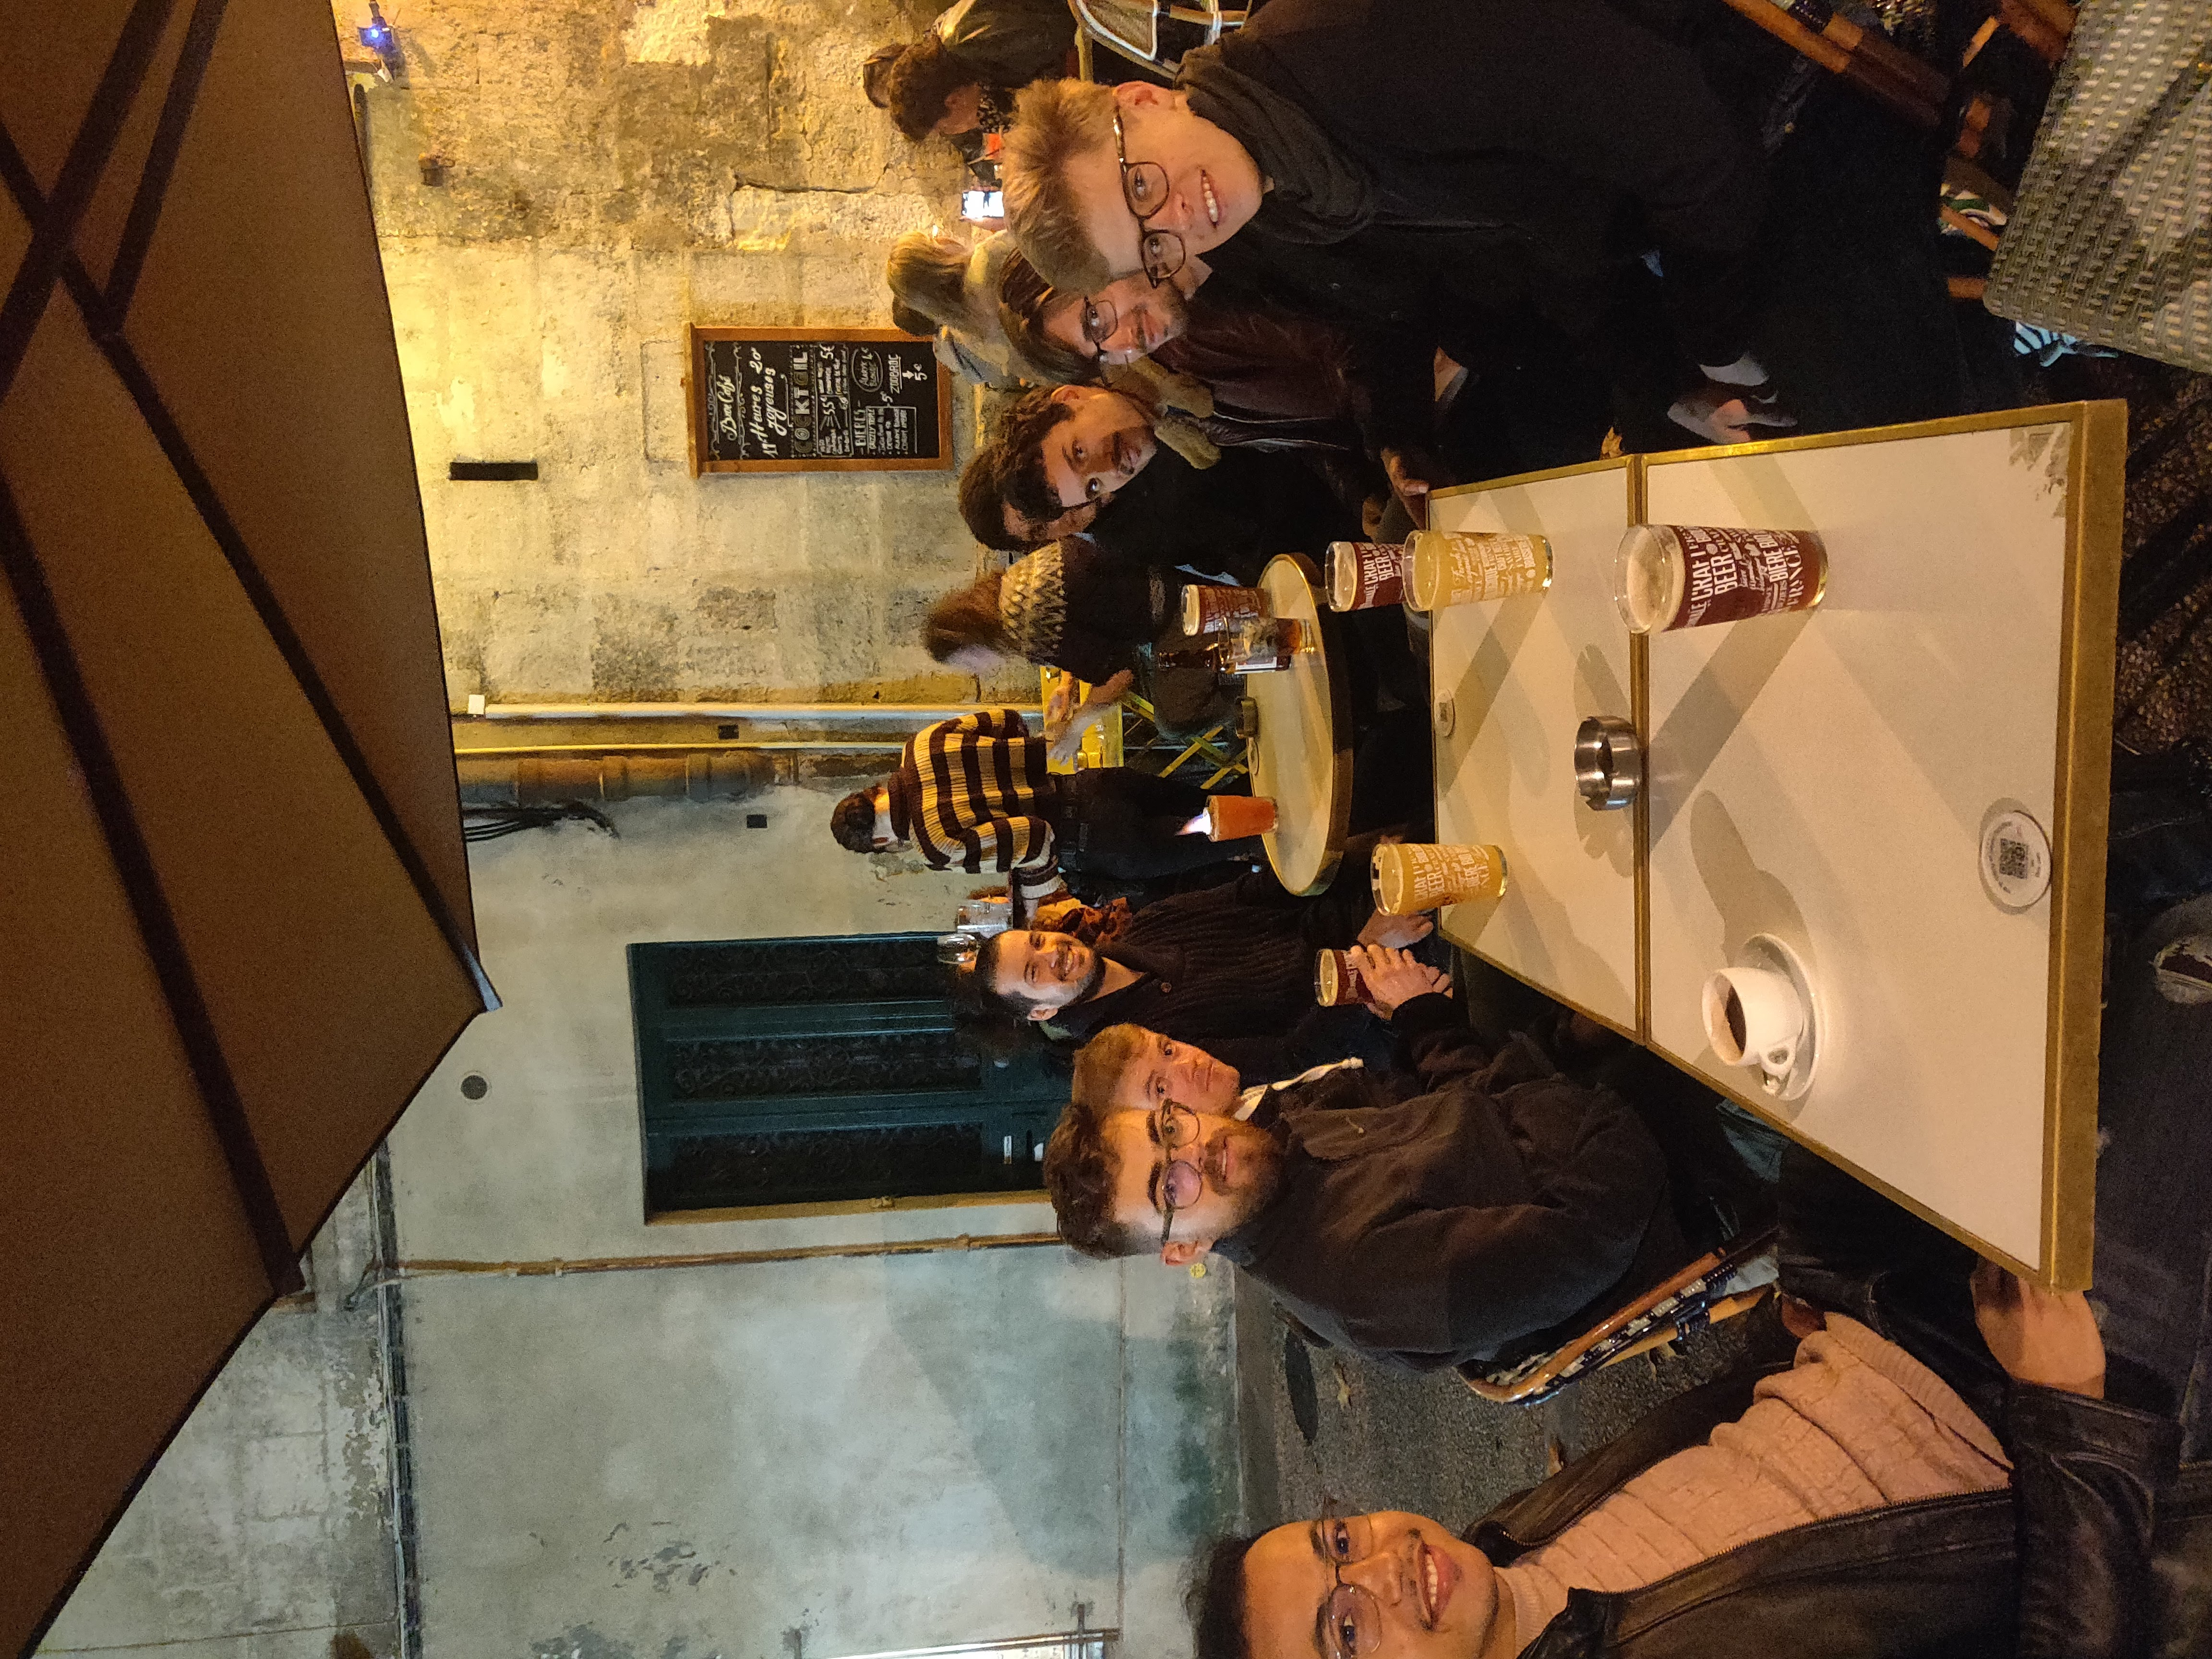
\includegraphics[width=.3\textwidth]{sharedimages/bar1.jpg}
    \\[-3em]
    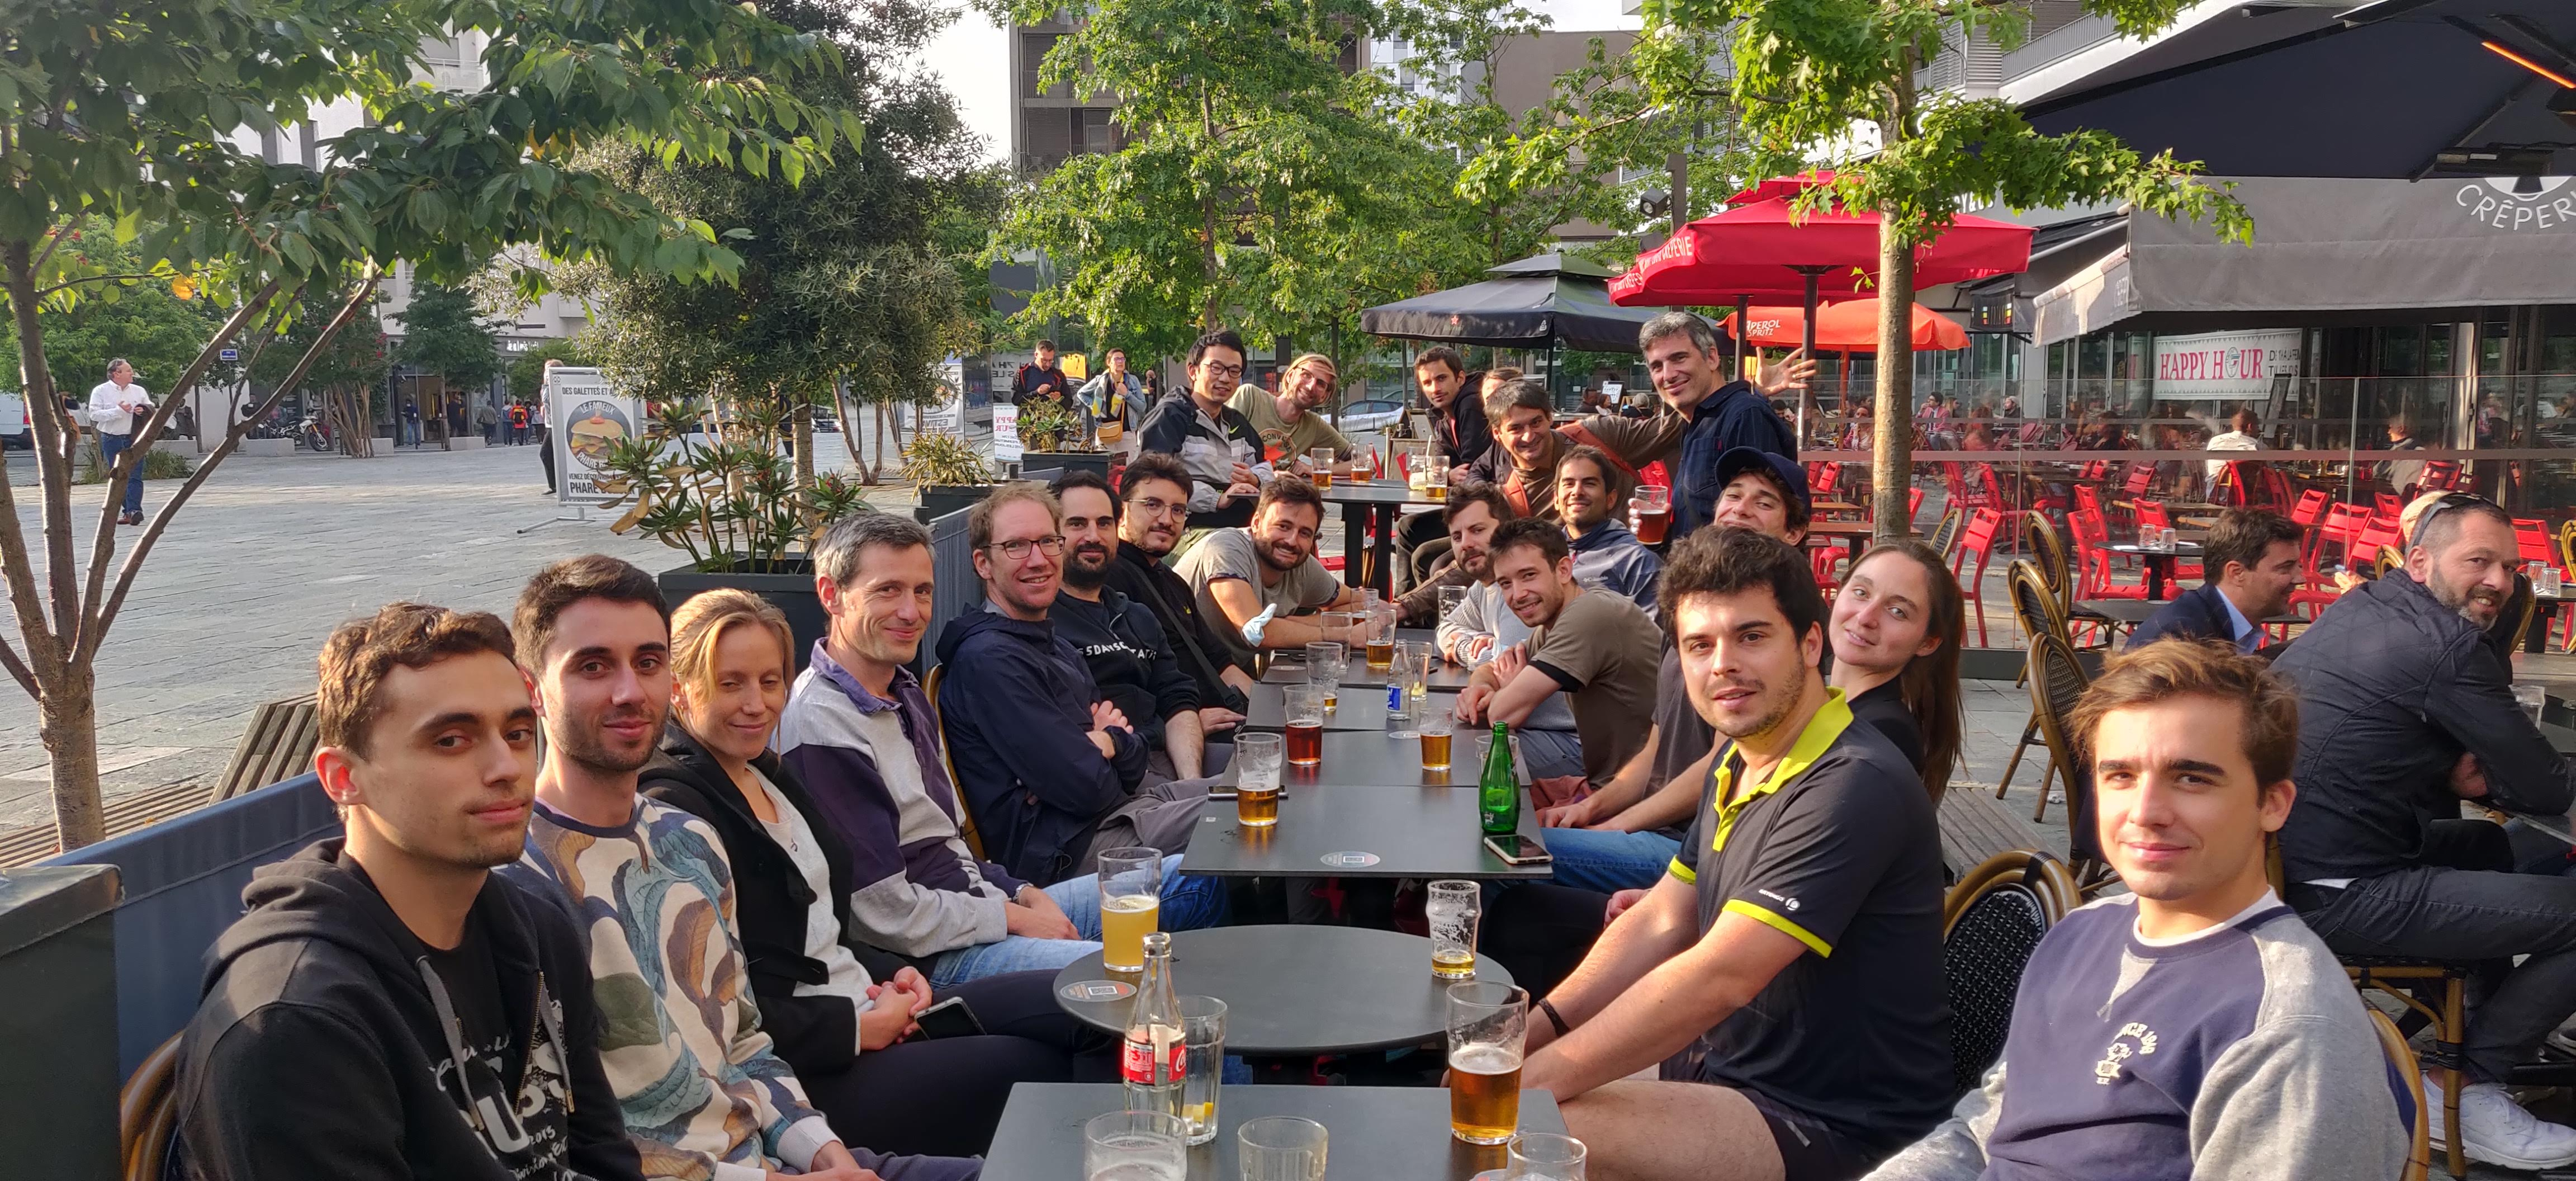
\includegraphics[width=.5\textwidth]{sharedimages/parietal_retreat.jpg}\\[-3em]
    \parbox[c]{.4\textwidth}{
        \centering \emph{Deep} Generative Modeling\\
        Physiological signals\\
        Point processes\\

    }\hfill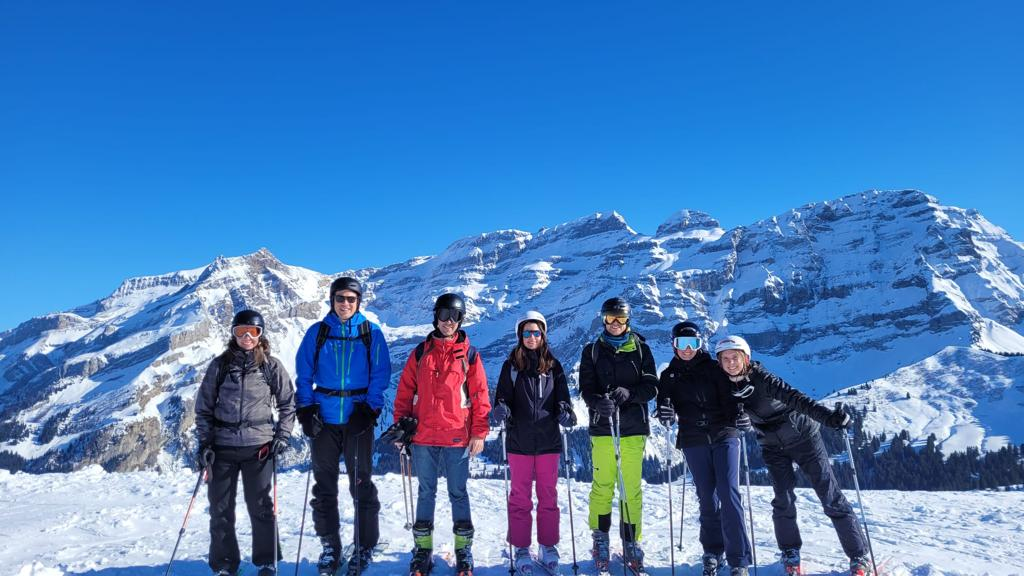
\includegraphics[width=.5\textwidth]{sharedimages/parietal_ski.jpg}\\


\end{frame}
%%%%%%%%%%%%%%%%%%%%%%%%%%%%%%%%%%%%%%%%%%%%%%%%%%%%%%%%%%%%%%%%%%%%%%%%%%%%%%%


\end{document}
